
\begin{figure}[tb]\centering
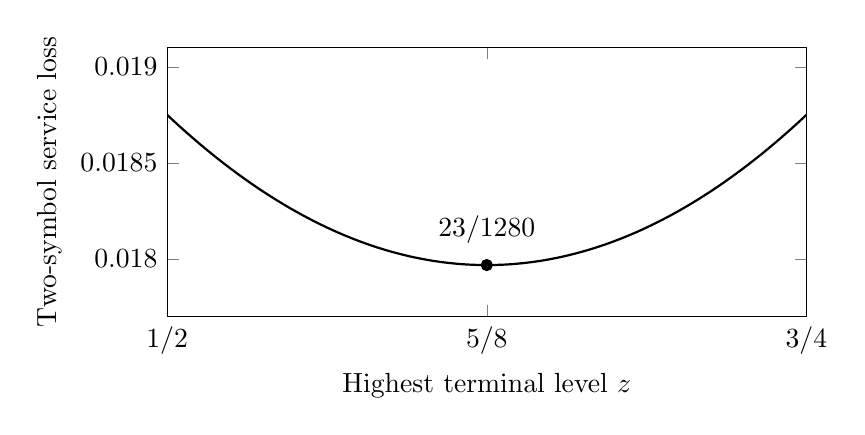
\begin{tikzpicture}
\begin{axis}[width=.8\textwidth,height=5cm,xlabel={Highest terminal level $z$},
 ylabel={Two-symbol service loss},xmin=.5,xmax=.75,ymin=.0177,ymax=.0191,
 scaled y ticks=false,yticklabel style={/pgf/number format/fixed,/pgf/number format/precision=4},
 xtick={.5,.625,.75},xticklabels={$1/2$,$5/8$,$3/4$}]
\addplot[domain=.5:.75,samples=101,thick]{x*x/20-x/16+3/80};
\addplot[only marks] coordinates {(.625,.01796875)};
\node[anchor=south] at (axis cs:.625,.01803) {$23/1280$};
\end{axis}\end{tikzpicture}
\caption{The analytically optimized highest level in the heterogeneous three-branch example. The lower level is $1/4$. The displayed function is $z^2/20-z/16+3/80$ on $[1/2,3/4]$; its interior minimum is $z=5/8$, not a branch cap.}\label{fig:top-loss}
\end{figure}
